\chapter{Émission et réception des ondes}
\section{Émission}
Créer une onde est simple : un courant alternatif est une oscillation de très faible 
amplitude des électrons à une fréquence donnée. Nous allons décrire l'émission en 
trois zones : proche, moyenne et lointaine (ce qui nous intéresse).

	\subsection{Champs rayonnés par un élément de courant}
	\begin{wrapfigure}[5]{r}{3.5cm}
	\vspace{-20mm}
	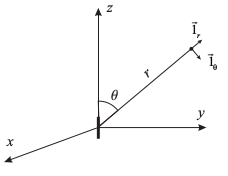
\includegraphics[scale=0.45]{ch4/image1.png}
	\captionof{figure}{ }
	\end{wrapfigure}
	Dans un fil les électrons vont un peu osciller et générer une petite onde. 
	Considérons un élément de courant, calculons les potentiels retardés et 
	sommons tous ces éléments. Un tel élément est un \textbf{dipôle}\footnote{"Pôle!"} 
	\textbf{de Hertz}. En considérant $\underline{I}\vec{1_z} = \underline{J}S\vec{1_z}$ 
	\begin{equation}
	\underline{\vec{A}}(\vec{r}) = \dfrac{\mu_0}{4\pi}\int_{-l/2}^{l/2} 
	\underline{I}\vec{1_z} \dfrac{e^{-j\beta|\vec{r}-\vec{r'}|}}{|\vec{r}-\vec{r'}|}\ dl'
	\end{equation}
	où $\vec{r'}$ est la coordonnée d'intégration, $\vec{r}$ le point de calcul et 
	$|\vec{r}-\vec{r'}|$ la distance entre le point d'intégration et le point de calcul.
	Comme le volume de l'élément de courant est petit comme ta \dots, nous ferons 
	l'hypothèse $l\ll r \rightarrow |\vec{r}-\vec{r'}| \approx r$. En sortant le propagateur
	\begin{equation}
	\underline{\vec{A}}(\vec{r}) = \dfrac{\mu_0}{4\pi}\dfrac{e^{-j\beta r}}{r}\underline{I}l
	\vec{1_z}
	\end{equation}
	En sphérique, c'est plus pratique (ça rime!)
	\begin{equation}
	\underline{\vec{A}}(\vec{r}) = \dfrac{\mu_0}{4\pi}\dfrac{e^{-j\beta r}}{r}\underline{I}l
	\left(\cos\theta\vec{1_r}-\sin\theta\vec{1_\theta}\right)
	\end{equation}
	Fastidieux, mais donne
	\begin{equation}
	\begin{split}
	\underline{\vec{B}}(\vec{r},\omega) &= \rot \underline{\vec{A}}(\vec{r},\omega)\\
	&=\dfrac{1}{r}\left(\dfrac{\partial}{\partial r}(r\underline{A}_\theta)-\dfrac{\partial 
	\underline{A}_r}{\partial \theta}\right)\vec{1_\phi}\\
	&= j\beta\underline{I}\sin\theta\dfrac{\mu_0}{4\pi}\dfrac{e^{-j\beta r}}{r}\left(1+
	\dfrac{1}{j\beta r}\right)\vec{1_\phi}
	\end{split}
	\end{equation}
	Remarquons que le champ étant en $\vec{1_\phi}$, celui-ci "tourne" autour de l'élément 
	de courant.	Le champ électrique s'obtient avec les équations de Maxwell : 
	$\underline{\vec{E}}(\vec{r},\omega) = \frac{1}{j\omega\epsilon_0\mu_0}\rot\underline{
	\vec{B}}(\vec{r},\omega)$. En considérant l'expression sphérique du rotationnel, on 
	trouve
	\begin{equation}
	\begin{split}
	\underline{E}_\theta &= j\dfrac{Z_0\beta\underline{I}l}{4\pi}\sin\theta\dfrac{e^{-j\beta r}}{
	r} \left(1+\dfrac{1}{j\beta r}-\dfrac{1}{(\beta r)^2}\right)\\
	\underline{E}_r &= \dfrac{Z_0\underline{I}l}{2\pi}\cos\theta \dfrac{e^{-j\beta r}}{r^2}
	\left(1+\dfrac{1}{j\beta r}\right)
	\end{split}
	\end{equation}
	où $Z_0$ est l'\textbf{impédance du vide} (historiquement, l'impédance de l'éther)\\
	
	\retenir{
	\begin{equation}
	Z_0=\sqrt{\dfrac{\mu_0}{\epsilon_0}}= 120\pi \approx 377\ \Omega
	\end{equation}}\ 
	
	Cette fois-ci le champ possède deux composantes : une radiale et une en $\theta$. 
	On s'intéresse souvent au cas \textit{loin de l'antenne} ; $\beta r \rightarrow\infty$. 
	En ne gardant que les termes dominant\footnote{Et avec une ré-écriture du sinus à l'aide 
	d'un produit vectoriel.} (soit celui en $1/r$)
	\retenir{\ \textbf{Région de champ lointain}
	\begin{equation}
	\begin{split}
	\underline{\vec{E}}(\vec{r}) &= j\omega \dfrac{\mu_0}{4\pi}\dfrac{e^{-j\beta r}}{r}
	\underline{I}l\sin\theta  \vec{1_\theta} = -j\omega \underline{A}_\theta\vec 1_\theta\\
	\underline{\vec{B}}(\vec{r}) &= \dfrac{1}{c}\left(\vec{1_r}\times\underline{\vec{E}}
	\right)
	\end{split}
	\end{equation}
	Les composantes de ces champs sont les \textit{champs rayonnés}.}\ \\
	
	Proche de l'élément les termes en $1/r^2$ et $1/r^3$ dominent le bazar et lah les champs 
	rayonnés : \textbf{région de champ proche}. Quel est la limite ? Si $\beta r= 1$, le 
	module des termes entre parenthèses de $B$ et $E$ est identique 
	\begin{equation}
	r = \dfrac{\lambda}{2\pi}
	\end{equation}
	Il s'agit de la limite de zone quasi-statique. Autour de n'importe quelle antenne, il 
	existe une zone où les délais de propagation sont si court qu'on considère le cas 
	quasi-statique : il s'agit de la zone de champ proche. Cette limite dépassée, nous 
	entrons dans la zone de champ lointain mais en dessous de celle-ci, il n'y a pas d'onde.
	Par exemple, il faut passer $r=\SI{5}{\meter}$ d'une voiture pour que celle-ci soit réellement 
	déverrouillée par des ondes. En dessous de cette distance, on retrouve le cas quasi-statique 
	et donc plus vraiment des ondes.\\
	
	Notre expression est généralisable en considérant $
	\sin\theta \vec{1_\theta} = \left(\vec{1_z}\times\vec{1_r}\right)\times\vec{1_r}$ tel que
	\begin{equation}
	\underline{\vec{E}}(\vec{r}) = j\omega\left(\underline{\vec{A}}\times\vec{1_r}\right)\times 
	\vec{1_r}
	\end{equation}
	Quatre observations
	\begin{enumerate}
	\item Les champs rayonnés sont purement transverses ($\theta,\phi$, rien en $r$)
	\item Le champ magnétique rayonné est perpendiculaire au champ électrique rayonné
	\item Les champ rayonné sont $\propto \omega$ : il est nécessaire d'utiliser de hautes 
	fréquences pour avoir des ondes sinon le rayonnement est trop faible
	\item T'es moche
	\end{enumerate}
	Remarquons également que $E\propto I$ : pour produire des ondes il faut du courant, et 
	un max plz!
	
	\subsection{Champs rayonnés par une distribution de courant}
	On a su exprimer $E = f(A)$, il n'y a plus qu'à appliquer le principe de superposition. 
	Reprenons l'expression générale
	\begin{equation}
	\underline{\vec{A}}(\vec{r}) = \dfrac{\mu_0}{4\pi}\int_\mathcal{D}\underline{\vec{J}}(\vec{r'})
	\dfrac{e^{-j\beta|\vec{r}-\vec{r'}|}}{|\vec{r}-\vec{r'}|}\ dV'
	\end{equation}
	À très grande distance par rapport au circuit émetteur, nous avions $|\vec{r}-\vec{r'}|
	\approx r$ pour le dénominateur du propagateur mais \textbf{pas} pour le terme de phase 
	à cause du produit par $\beta = 2\pi/\lambda$. Il suffit dès lors de remarquer que, dans le 
	champ lointain, $\vec{r}$ et $\vec{r}-\vec{r'}$ sont quasiment parallèle :
	\begin{equation}
	|\vec{r}-\vec{r'}| \approx r - \vec{r'}.\vec{1}_r
	\end{equation}

\begin{center}
	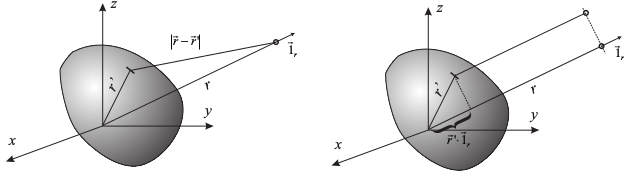
\includegraphics[scale=0.45]{ch4/image2.png}
	\captionof{figure}{ }
\end{center}

	Le terme de phase devient
	\begin{equation}
	e^{-j\beta|\vec{r}-\vec{r'}|} \approx e^{-j\frac{2\pi}{\lambda}r}\ e^{j2\pi\frac{\vec{r'}.\vec{1}_r}{
	\lambda}}
	\end{equation}
	Le deuxième terme est négligeable si les dimensions du circuit émetteur sont petites par rapport 
	à la longueur d'onde : $r' \ll \lambda$ (généralement pas le cas). Dès lors
	\begin{equation}
	\underline{\vec{A}}(\vec{r}) = \dfrac{\mu_0}{4\pi}\dfrac{e^{-j\beta r}}{r}\int_\mathcal{D}
	\underline{J}(\vec{r'})e^{j\beta(\vec{r'}.\vec{1_r})}\ dV'
	\end{equation}
	Le rayonnement peut être caractérisé par une grandeur dépendant de la direction ($\theta,\phi$) 
	mais pas de la distance. La directionalité (le gain) est alors \textbf{indépendant} de la 
	distance à la quelle on se trouve du circuit. On définit alors\\
	
	\retenir{
	\begin{equation}
	\vec{A}^\circ(\theta,\phi) = \dfrac{\mu_0}{4\pi}\int_\mathcal{D}\underline{J}(\vec{r'})
	e^{j\beta(\vec{r'}.\vec{1_r})}\ dV'
	\end{equation}}\ \\
	
	La connaissance de $\vec{A}^\circ(\theta,\varphi)$ permet de tout déduire : pour une antenne, 
	on parlera de \textit{diagramme de rayonnement} (de cette antenne). Les éléments de courants 
	ne sont pas tous au même endroit, mais pour $r\rightarrow\infty$ on peut grosso-modo considérer 
	que oui pour obtenir\\
	\retenir{\begin{equation}
	\begin{aligned}
	\underline{E}_r &= 0\\
	\underline{E}_\theta &= -j\omega\underline{A}_\theta &= -j\omega A_\theta^\circ(\theta,\phi)
	\frac{e^{-j\beta r}}{r}\\
	\underline{E}_\phi &= -j\omega\underline{A}_\phi &= -j\omega A_\phi^\circ(\theta,\phi)
	\frac{e^{-j\beta r}}{r}	
	\end{aligned}
	\end{equation}}\ 
	
	On peut en déduire le champ magnétique rayonné $\left(\underline{\vec{B}}(\vec{r}) = 
	\frac{1}{c}\left(\vec{1_r}\times\underline{\vec{E}}\right)\right)$. Pour obtenir ce résultat, 
	nous avons du faire une approximation : intéressons nous à la validité de celle-ci. Sans 
	approximation, nous avons (au premier ordre)
	\begin{equation}
	|\vec{r}-\vec{r'}| = \sqrt{(\vec{r}-\vec{r'}).(\vec{r}-\vec{r'})} = r\sqrt{1-2\frac{\vec{r}.
	\vec{r'}}{r^2}+\frac{r^{'2}}{r^2}} \approx r-\vec{r'}.\vec{1_r}+\frac{r^{'2}}{2r}
	\end{equation}
	Cette approximation génère une erreur de $\frac{r^{'2}}{2r}$. Historiquement, on la définit 
	\textit{acceptable} tant qu'elle n'excède pas $\pi/8$ (\danger ne pas oublier $\beta$)
	\begin{equation}
	\beta\frac{r^{'2}}{2r} < \frac{\pi}{8}
	\end{equation}
	Comme $r'\lesssim D/2$ où $D$ est la dimension caractéristique maximale du circuit, on obtient\\
	\retenir{\ \textbf{Zone de Fraunhofer}\begin{equation}
	r > \dfrac{2D^2}{\lambda}
	\end{equation}}\ \\
	
	\danger Cette zone est celle ou l'approximation du champ lointain peut être utilisé pour 
	calculer les champs rayonnés et \textbf{non pas} celle ou les champ rayonnés sont prédominants 
	(région de champ lointain)
	
\section{Théorème de Poynting}
	\subsection{Discussion physique}
Séparer des masses demande une certaine énergie potentielle. De même dans un condensateur, pour 
séparer les charges + et -, il faut fournir de l'énergie. Par conservation de l'énergie, lorsqu'un 
champ rayonné se "détache" de sa source il vit sa propre vie indépendamment de si la source est 
allumée ou éteinte et "emporte" avec lui de l'énergie. Ce théorème permet de calculer celle-ci sous 
la forme d'un bilan (conservation de l'énergie. Schéma++ à l'examen\footnote{\cancel{Voir feuille Cédric}}).\\

Avant, cherchons la forme d'un tel bilan dans un espace $\mathcal{D}$. La densité volumique 
d'énergie totale dans les champs vaut
\begin{equation}
w(\vec{r},t) = \dfrac{\epsilon|\vec{E}|^2}{2}+\dfrac{|\vec{B}|^2}{2\mu}
\end{equation}
La variation temporelle d'énergie vaut alors
\begin{equation}
\dfrac{dW}{dt} = \dfrac{d}{dt}\int_\mathcal{D}\dfrac{\epsilon|\vec{E}|^2}{2}+\dfrac{|\vec{B}|^2}{2\mu}
\ dV
\end{equation} 
Qu'est ce qui peut produire cette variation? La puissance de la source $P_S$ fournie des sources 
aux charges (transfo. chimique/mécanique). La puissance $P_J$ dissipée par effet Joule, correspondant 
à une perte. Enfin, l'énergie pouvant entrer et sortir de $\mathcal{D}$ délimité par $S$ (par exemple 
via un champ rayonné de puissance $P_r$\footnote{Positive si quitte $\mathcal{D}$.}. Mathématiquement
\begin{equation}
\dfrac{dW}{dt} = P_S(t)-P_J(t)-P_r(t)\qquad\Leftrightarrow\qquad P_r(t)+\dfrac{dW}{dt} = P_S(t)-P_J(t)
\end{equation}
À droite : \textit{transformation}	d'énergie vers ou depuis les champs. À gauche : bilan est soit 
emmagasiné dans $\mathcal{D}$ soit transporté vers (ou depuis) l'extérieur à travers $S$.
	
	\subsection{Démonstration}
	Intéressons nous à l'effet du champ ambiant sur les $e^-$. Multiplions scalairement par la vitesse
	\begin{equation}
	\vec{F} = q(\vec{E}+\vec{v}\times\vec{B})\qquad \Leftrightarrow\qquad \vec{F}.\vec{v}=q\vec{E}.
	\vec{v}
	\end{equation}
	Nous avons $N$ charges. Sachant que $Nqv = J$
	\begin{equation}
	Nq\vec{E}.\vec{v} = \vec{E}.\vec{J}
	\end{equation}
	Il faut distinguer le cas des conducteurs et des sources pour calculer $\vec{E}.\vec{J}$. 
	\begin{itemize}
	\item \textit{Conducteur} : $\vec{J}=\sigma\vec{E}$, $\vec{E}.\vec{J} = \sigma|\vec{E}|^2=
	\frac{|\vec J|^2}{\sigma}$. Cette densité ($\vec{E}.\vec{J}$) est transformée sous forme 
	de chaleur.
	\item \textit{Source} : $\vec{E}.\vec{J}<0$, le champ gagnant en puissance (la source 
	fait "remonter" les charges du potentiel). Ceci est possible grâce à une force non-EM. Soit 
	$\vec{f_S}$ cette force par unité de charge. Le cours d'\textit{Électricité} nous dis que
	\begin{equation}
	\vec{f_S} = -\vec{E}+\dfrac{\vec{J}}{\sigma}
	\end{equation}
	Dans un source
	\begin{equation}
	-\vec{E}.\vec{J} = \vec{f_S}.\vec{J}-\dfrac{|\vec{J}|^2}{\sigma}
	\end{equation}
	où le membre de gauche correspond au champ et le membre de droite à la source (origine non EM 
	diminuée par la puissance dissipée).
	\end{itemize}		
	La puissance totale \textit{gagnée} par les champs dans $\mathcal{D}$ vaut
	\begin{equation}
	\int_\mathcal{D}(-\vec{E}.\vec{J}).dV = \underbrace{\int_\mathcal{D}\vec{f_S}.\vec{J}\ dV}_{=P_S}
	-\underbrace{\int_\mathcal{D}\dfrac{|\vec{J}|^2}{\sigma}\ dV}_{=P_J}
	\end{equation}
	Cette intégrale donne $P_S-P_J$. On peut calculer cette intégrale grâce à une astuce 
	vectorielle (pas connaître par cœur)(on peut le démontrer mais c'est pas super important, 
	dit-il en rigolant). Après avoir fait les math
	\begin{equation}
	\int_\mathcal{D}(-\vec{E}.\vec{J})dV = \oint_S\left(\dfrac{1}{\mu}\vec{E}\times\vec{B}\right)
	.\vec{dS} + \dfrac{d}{dt}\int_\mathcal{D}\left(\dfrac{\epsilon|\vec{E}|^2}{2}+\dfrac{|\vec{B}|^2}
	{2\mu}\right)\ dV
	\end{equation}
	Si $P_r(t) := \displaystyle\oint_S\left(\dfrac{1}{\mu}\vec{E}\times\vec{B}\right).\vec{dS}$ alors on retrouve 
	bien le membre de gauche de notre équation de bilan. On défini\\
	\retenir{\ \textbf{Vecteur de Poynting}\begin{equation}
	\vec{S}(\vec{r},t) = \dfrac{1}{\mu}\vec{E}(\vec{r},t)\times\vec{B}(\vec{r},t)
	\end{equation}}\ 
	
	Avec la ré-écriture
	\begin{equation}
	P_r(t) = \oint_S \vec{S}(\vec{r},t).\vec{dS}
	\end{equation}
	On obtient la forme finale du théorème de Poynting \\
	\theor{\begin{equation}
	\oint_S \vec{S}(\vec{r},t).\vec{dS}+\dfrac{dW}{dt} = P_S(t)-P_J(t)
	\end{equation}
	La puissance entrant/sortant de $\mathcal{D}$ est donnée par le flux du vecteur de Poynting 
	à travers $S$.}\ \\
	
	On peut extrapoler et dire que le vecteur de Poynting $\vec{S}$ représente \textit{localement} 
	la densité de puissance transportée : tous les transferts d'énergie se font via ce vecteur. Sa 
	norme donne une densité de puissance et son orientation la direction de propagation de l'énergie. 
	
	
	\subsection{Régime sinusoïdal permanent}
	On notera la moyenne sur une période < . >. Exprimons les champs en phaseur
	\begin{equation}
	\begin{aligned}
	\vec{E}(\vec{r},t) &= \Re\left(\underline{\vec{E}}e^{j\omega t}\right) &= \dfrac{1}{2}\left(
	\underline{\vec{E}}e^{j\omega t}+\underline{\vec{E}}^*e^{-j\omega t}\right)\\
	\vec{B}(\vec{r},t) &= \Re\left(\underline{\vec{B}}e^{j\omega t}\right) &= \dfrac{1}{2}\left(
	\underline{\vec{B}}e^{j\omega t}+\underline{\vec{B}}^*e^{-j\omega t}\right)
	\end{aligned}
	\end{equation}
	Par multiplication vectorielle
	\begin{equation}
	\vec{E}(\vec{r},t)\times\vec{B}(\vec{r},t) = \frac{1}{4}\underline{\vec{E}}\times\underline{
	\vec{B}}e^{2j\omega t} +\frac{1}{4}\underline{\vec{E}}\times\underline{\vec{B}}^* + \frac{1}{4}
	\underline{\vec{E}}^*\times\underline{\vec{B}}+\frac{1}{4}
	\underline{\vec{E}}^*\times\underline{\vec{B}}^* e^{-2j\omega t}
	\end{equation}
	Les termes ayant une dépendance temporelle ont une moyenne nulle sur une période\footnote{Les 
	exponentielle pouvant être vues comme "constantes au niveau du temps"} :
	\begin{equation}
	\vec{\mathcal{S}}(\vec{r},\omega) = \frac{1}{\mu}\langle\vec{E}\times\vec{B}\rangle 
	=\dfrac{1}{4\mu}\underline{\vec{E}}\times\underline{\vec{B}}^* + \frac{1}{4\mu}
	\underline{\vec{E}}^*\times\underline{\vec{B}}
	\end{equation}
	
	\retenir{\begin{equation}
	\vec{\mathcal{S}}(\vec{r},\omega) = \dfrac{1}{2\mu}\Re\left(
	\underline{\vec{E}}\times\underline{\vec{B}}^*\right)
	\end{equation}
	Soit le vecteur de Poynting (valeur moyenne et \textbf{non} instantanée)}\ 
	
	Dans le champ lointain ($\vec{B} = \frac{1}{c}\vec{1_r}\times\vec{E}$ dans 
	l'expression ci-dessus) l'expression se simplifie. La puissance totale est donnée par 
	l'intégration du vecteur de Poynting sur toute surface fermée entourant le circuit\footnote{
	Soit le flux du vecteur de Poynting} :\\
	\retenir{\begin{equation}
	\vec{\mathcal{S}}(\vec{r},\omega) = \dfrac{1}{2Z_0}|\underline{\vec{E}}|^2\vec{1_r},\qquad\qquad\qquad
	P_r = \oint_S \vec{\mathcal{S}}(\vec{r},\omega)\ .\ \vec{dS}
	\end{equation}}
	
	\subsection{Puissance rayonnée par un élément de courant}
	Comme notre vecteur de Poynting est en $\vec{1_r}$, choisissons une surface ou le produit 
	scalaire $\vec{\mathcal{S}}.\vec{dS}$ est simple (soit parallèle à ce vecteur) : intégrons 
	sur une sphère de rayon $r$ centrée sur l'élément
	\begin{equation}
	\begin{split}
	P_r = \oint_S \vec{\mathcal{S}}(\vec{r},\omega)\ .\ \vec{dS}  &= \int_0^{\pi}\int_0^{2\pi}
	\vec{\mathcal{S}}.\vec{1_r}r^2\sin\theta d\theta d\phi\\
	&= \dfrac{2\pi}{2Z_0}\left(\dfrac{\mu_0|\underline{I}|l\omega}{4\pi}\right)^2 \int_0^\pi 
	\dfrac{\sin^2\theta}{r^2}r^2\sin\theta d\theta\\
	&= \dfrac{1}{12\pi Z_0}\left(\omega\mu_0|\underline{I}|l\right)^2
	\end{split}
	\end{equation}
	Remarquons la simplifications des $r^2$ : sans celle-ci, cela voudrait dire que la puissance 
	observée dépendrait de la distance de la source ce qui est absurde. Ceci donne la justification 
	du terme en $1/r$ du propagateur, nécessaire à la conservation de l'énergie. Ce terme n'est 
	donc pas une atténuation mais une "\textit{dilution}". Remarquons que la puissance rayonnée 
	dépend du carré de la fréquence, mais également du courant.
	
\section{Réception}
Pour détecter un courant, $\underline{\vec{E}}_i$ de l'onde incidente doit mettre les $e^-$ 
en oscillation : un élément $\vec{dl}$ est soumis à une tension $\underline{\vec{E}}_i.\vec{dl}$ générant 
un courant $\underline{I}\vec{dl}$. N'oublions cependant pas que ce champ ne fait que propager 
l'information (interaction entre charges) du circuit émetteur à récepteur. On pourrait 
vouloir utiliser $q\vec{v}\times\vec{B}$ mais c'est mort sans vitesse. Il va falloir ruser.

	\subsection{Le théorème de réciprocité}
	Ce théorème ne sera pas démontré. Considérons deux circuits rayonnants à deux accès : 
	équivalent à un biporte
	\begin{equation}
	\left\{\begin{array}{ll}
	\underline{V}_1 &= Z_{11}\underline{I}_1 +Z_{12}\underline{I}_2\\
	\underline{V}_2 &= Z_{21}\underline{I}_1 +Z_{22}\underline{I}_2	
	\end{array}\right.\qquad\Leftrightarrow\qquad
	\left\{\begin{array}{ll}
	\underline{I}_1 &= Y_{11}\underline{V}_1 + Y_{12}\underline{V}_2\\
	\underline{I}_2 &= Y_{21}\underline{V}_1 + Y_{22}\underline{V}_2	
	\end{array}\right.
	\end{equation}
	\begin{center}
	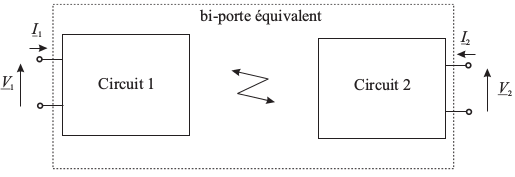
\includegraphics[scale=0.45]{ch4/image3.png}
	\captionof{figure}{ }
	\end{center}
	Le théorème affirme que $Z_{12}=Z_{21}$ et donc $Y_{12}=Y_{21}$.
	
	
	\subsection{Calcul de la tension induite}
	\begin{wrapfigure}[4]{r}{4cm}
	\vspace{-15mm}
	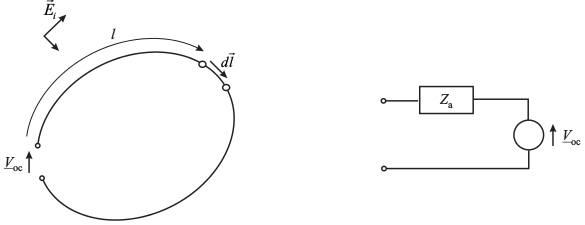
\includegraphics[scale=0.25]{ch4/image4.png}
	\captionof{figure}{ }
	\end{wrapfigure}
	Soit le circuit ci-contre d'impédance d'entrée $Z_a$. Quand $\underline{\vec{E}}_i$ se frah 
	sur lui, une tension $\underline{V}_{oc}$ est induite : nous la cherchons. Appliquons le 
	théorème de réciprocité sur un élément $\vec{dl}$ à distance $l$ de l'accès\footnote{Le courant 
	est considéré comme une grandeur locale $\underline{I}(l)$ hors quasi-statique.}. Voyons 
	trois cas :
	\begin{enumerate}
	\item Appliquons $\underline{V}_a$ à l'accès \textbf{sans} champ incident $\underline{\vec{E}}_i$. 
	Un courant $\underline{I}(l)$ circule dans $\vec{dl}$, le circuit est un \textit{émetteur}. Par 
	Thévenin 
	\begin{equation}
	\underline{I}_a = \dfrac{\underline{V}_a}{Z_a}
	\end{equation}
		\begin{center}
	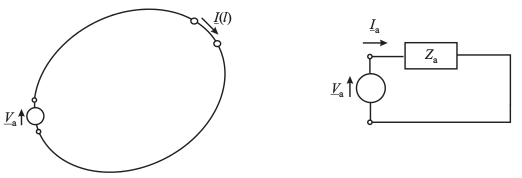
\includegraphics[scale=0.45]{ch4/image5.png}
	\captionof{figure}{ }
	\end{center}
	\item Un rayonnement extérieur $\underline{\vec{E}}_i$ est présent : récepteur. La tension appliquée 
	en $l$ vaut $\underline{\vec{E}}_i(l).\vec{dl}$. Par Thévenin, c'est équivalent à une source de 
	tension $\underline{dV}_{oc}$ placée à cet endroit.
			\begin{center}
	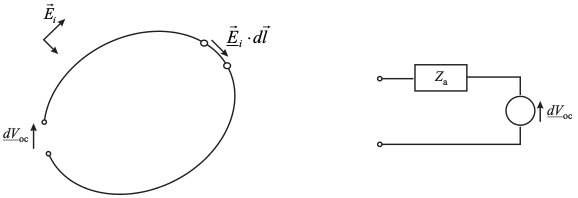
\includegraphics[scale=0.45]{ch4/image6.png}
	\captionof{figure}{ }
	\end{center}
	\item Court-circuit : courant $\underline{dI}_{sc}$. Par Thévenin
	\begin{equation}
	\underline{dI}_{sc} = -\dfrac{\underline{dV}_{oc}}{Z_a}
	\end{equation}
			\begin{center}
	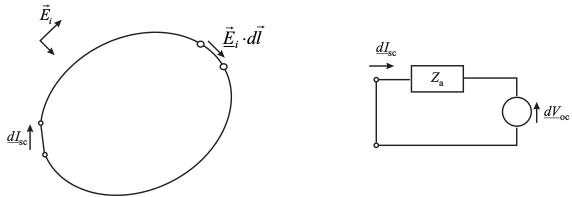
\includegraphics[scale=0.45]{ch4/image7.png}
	\captionof{figure}{ }
	\end{center}
	\end{enumerate}
	Par application du théorème de réciprocité
	\begin{equation}
	\dfrac{\underline{I}(l)}{\underline{V}}_a = \dfrac{\underline{dI}_{sc}}{\underline{\vec{E}}_i(l).
	\vec{dl}}\qquad\text{ ou }\qquad
	\dfrac{\underline{I}(l)}{\underline{I}}_a = \dfrac{-\underline{dV}_{oc}}{\underline{\vec{E}}_i(l).
	\vec{dl}}
	\end{equation}
	Dès lors
	\begin{equation}
	\underline{dV}_{oc} = -\dfrac{1}{\underline{I}_a}\underline{I}(l)\underline{\vec{E}}_i(l).\vec{dl}
	\end{equation}
	La tension est la somme des tensions locale, mais cette somme est pondérée par la valeur du courant 
	que l'on trouverait à ce point là \textbf{si le circuit fonctionnait en émetteur}:\\
	\retenir{\begin{equation}
	\underline{V}_{oc} = -\dfrac{1}{\underline{I}_a}\int_c \underline{I}(l)\underline{\vec{E_i}}(l).\vec{dl}
	\end{equation}
	où $\underline{\vec{E}}_i(l)$ est le champ incident sur le circuit, $\underline{I}_a, \underline{I}(l)$ 
	sont les courant à l'accès et en $l$ si le circuit fonctionnait en \textbf{émission}.}